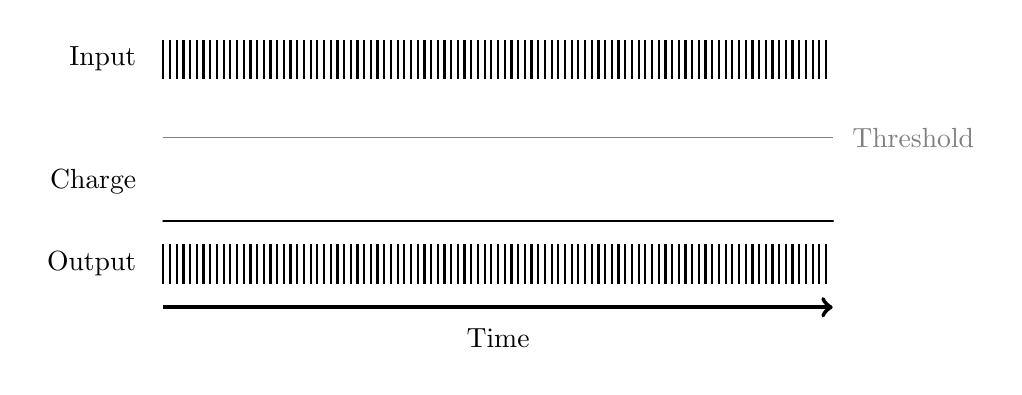
\begin{tikzpicture}[thick, xscale=0.085, inner sep=0.7em]
	\pgfmathsetseed{41}
	
	\pgfmathtruncatemacro{\duration}{100}
	\pgfmathsetmacro{\spikeprob}{0.1}
	
	% Threshold charge
	\pgfmathsetmacro{\threshold}{1.0}
	% Charge added by arrival of a spike
	\pgfmathsetmacro{\spikecharge}{0.5}
	% Decay rate of charge
	\pgfmathsetmacro{\chargedecay}{0.95}
	
	% Space between plots
	\pgfmathsetmacro{\plotspacing}{0.3}
	
	% Extra space above charge (for spike peaks to protrude)
	\pgfmathsetmacro{\chargeextra}{0.5}
	
	% Height of spikes drawn on the plot
	\pgfmathsetmacro{\spikeheight}{0.5}
	
	\pgfmathsetmacro{\neuroncharge}{0.0}
	\foreach \x in {1,...,\duration}{
		% Decay the charge
		\pgfmathsetmacro{\newcharge}{\neuroncharge * \chargedecay}
		
		% Output spike produced?
		\ifthenelse{\lengthtest{\newcharge pt > \threshold pt}}{
			% Spiked!
			\pgfmathsetmacro{\newcharge}{\newcharge - \threshold}
			
			% Draw the outgoing spike
			\draw (\x - 1, -\spikeheight - \threshold - 2*\plotspacing)
			      -- ++(0, \spikeheight);
			\pgfmathtruncatemacro{\spiked}{1}
		}{
			\pgfmathtruncatemacro{\spiked}{0}
		}
		
		% Update charge according to incoming spikes
		\pgfmathtruncatemacro{\spike}{floor(random()/\spikeprob)}
		\ifthenelse{\equal{\spike}{0}}{
			\pgfmathsetmacro{\newcharge}{\newcharge + \spikecharge}
			
			% Draw the incoming spike
			\draw (\x - 1, \chargeextra) -- ++(0, \spikeheight);
		}{}
		
		% Draw charge plot
		\ifthenelse{\equal{\spiked}{0}}{
			\draw [line cap=round] (\x-1, \neuroncharge - \threshold - \plotspacing)
			                    -- (\x, \newcharge - \threshold - \plotspacing);
		}{
			\coordinate (peak) at (\x-1, \neuroncharge - \threshold - \plotspacing);
			\draw [line cap=round] (peak) |- (\x, \newcharge - \threshold - \plotspacing);
		}
		
		% Remember charge for next time...
		\global\let\neuroncharge=\newcharge
	}
	
	% Threshold voltage
	\draw [help lines]
	      (0, -\plotspacing + 1/\chargedecay - 1) -- ++(\duration, 0)
	      node [anchor=west] {Threshold};
	
	% Time axis
	\draw [->, ultra thick]
	      (0, -\spikeheight -\threshold - 3*\plotspacing)
	      -- node [anchor=north] {Time}
	      ++(\duration+0, 0);
	
	\node at (-1, \chargeextra + 0.5*\spikeheight)
	      [anchor=east]
	      {Input};
	
	\node at (-1, 0.5*\neuroncharge - 0.5*\threshold - \plotspacing)
	      [anchor=east]
	      {Charge};
	
	\node at (-1, -0.5*\spikeheight - \threshold - 2*\plotspacing)
	      [anchor=east]
	      {Output};
	
	
\end{tikzpicture}
